\chapter{Trabalhos Relacionados}
\label{cha:related_work}

A seguir serão descritos brevemente alguns projetos que inspiraram a criação de Rivers não necessariamente relacionados à linguagem Go mas que aplicam conceitos similares para processamento de dados frequentemente no formato de streams.

\section{Apache Spark}
\label{sec:apache_spark}

Achache Spark \cite{docs:apache:spark} é uma solução para computação de tempo real, tolerante a falhas e com suporte a clustering \cite{article:kris:clustering}, com APIs em diferentes linguagens de programação como por exemplo scala, java e python. Spark tornou-se muito popular em áreas de \emph{Machine Learning} \cite{course:coursera:ml} e \emph{Analytics} \cite{article:techtarget:analytics} devido ao seu grande poder computacional que permite que grandes volumes de dados possam ser processados e distribuídos em diferentes máquinas de um cluster sendo uma solução muito atrativa também para sistemas de processamento de eventos \cite{docs:apache:streaming}.

\begin{figure}[H]
  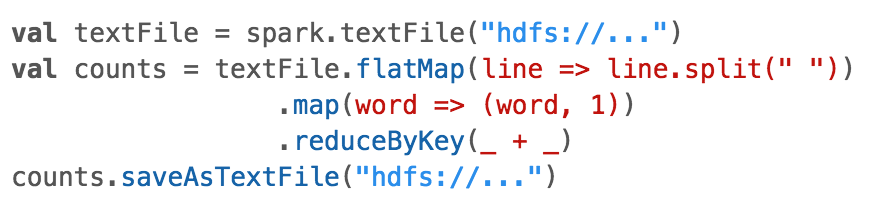
\includegraphics[width=0.7\textwidth]{spark}
  \centering
  \caption{Exemplo de uso da API scala de Spark.}
  \label{code:apache:spark}
\end{figure}

A API de Rivers é fortemente inspirada na fluência da API Spark, aplicando \emph{Method Chaining} \cite{article:sitepoint:method_chaining} sempre que possível aumentando a legibilidade do código resultante. Ambas APIs aplicam ao máximo os conceitos de programação funcional disponibilizando operações de filtros, mapeadores e agregadores de dados provendo um considerável nível de composição entre operações permitindo a criação de pipelines complexos de processamento de streams fortemente suscetíveis ao reuso. Suporte à clustering em Rivers é proposto como parte de trabalhos futuros.

\section{Java 8 Streams}
\label{sec:java8_streams}

A versão 8 da linguagem de programação Java introduz a abstração de Streams \cite{docs:java8:streams} como parte de suas bibliotecas padrão e assim como outras linguagens e plataformas como Spark, disponibiliza uma API fluente baseada em conceitos de programação funcional, permitindo a criação de pipelines para processamento de streams com suporte a paralelização. Assim como Spark, a API de streams de Java8 contribuíram para o design da API de Rivers afim de prover uma API similar para a linguagem Go que não fosse somente simples porém familiar à desenvolvedores com conhecimentos de programação funcional e extensível permitindo que a solução fosse aplicada à novos casos de uso introduzindo implementações diferentes dos componentes básicos do framework \ref{sec:rivers:building_blocks}.

\begin{figure}[H]
  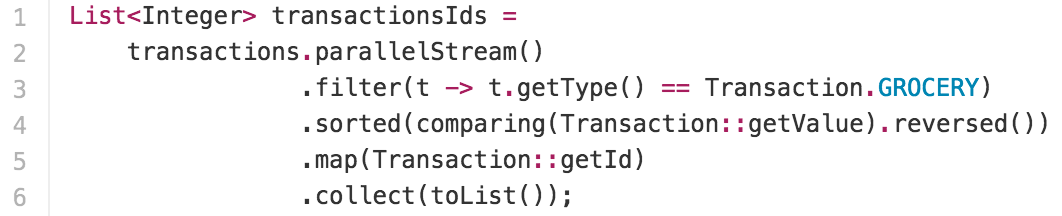
\includegraphics[width=0.9\textwidth]{java8_streams}
  \centering
  \caption{Exemplo de uso da API de streams em Java8.}
  \label{code:java8:streams}
\end{figure}

\section{ReactiveX - Reactive eXtensions}
\label{sec:reactive_extensions}

\emph{Reactive eXtensions} \cite{docs:reactivex:streams} é um movimento que tomou tração nos últimos anos liderado por empresas como \cite{netflix} e \cite{microsoft} dentre outras que procura tornar \emph{mainstream} conceitos de programação reativa \cite{article:reactive_programming} empregando vários conceitos de programação funcional e conhecidos padrões de design como \emph{Observer Pattern} \cite{article:pattern:observer} e \emph{Observable Pattern} \cite{article:pattern:observable} na criação de APIs assíncronas para tratamento de fluxo de dados. Estes conceitos quando combinados permitem com que APIs poderosas sejam implementadas abstraindo muito dos desafios envolvidos na programação assíncrona como por exemplo sincronização de threads, estruturas de dados concorrentes e operações de IO não bloqueantes. Existem várias implementações da especificação dentre elas estão a API Java \cite{docs:javarx} e Javascript \cite{docs:javascriptrx}.

Apesar de Rivers não seguir necessariamente a especificação de Reactive eXtensions, muitas decisões de design em Rivers foram baseados em conceitos similares aplicados à RX, como por exemplo realização de \emph{back-pressure} \cite{article:tim:streams} do pipeline através da utilização de Go \emph{buffered channels} \cite{docs:go:buffered_channels}. Reactive eXtensions e outros casos de uso explorados neste capítulo mostram que processamento de streams é uma solução interessante para muitos problemas relacionados a diversas áreas tecnológicas como por exemplo Big Data, Analytics, Event Processing e muitas linguagens de programação adotaram estes conceitos de provendo APIs nativas que permitem com que pipeline de processamento de streams sejam criados de maneira simples abstraindo muito dos desafios envolvidos com relação a concorrência e paralelização de um pipeline por exemplo, motivando a criação de Rivers.

\begin{flushright}
\mbox{}\vfill
{\sffamily\itshape
``ReactiveX is more than an API, it's an idea and a breakthrough in programming. It has inspired several other APIs, frameworks, and even programming languages.''\\}
--- \textsc{ReactiveX.io}
\end{flushright}
